Let's begin with some background knowledge.\\
Blockchain is a decentralized digital ledger in which data can be written and recorded chronologically and publicly.
In other words, blockchain is a protocol for a distributed database, continuously reconciled by millions of miners.
Miners are the computers that power this decentralized database.
When a user wishes to write data, he uses the blockchain's proprietary protocol to broadcast his action on the database
to the network of miners.
There, the miners pool many of these operations (e.g. transactions or contracts) into a computer data structure called a block,
and then compute a pre-defined (by the blockchain) arbitrary problem with this block as input,
that is known to be computationally expensive.
Discussion beyond basic concept of these computational so-called 'proof-of-work' is not necessary at this point.
The first miner to find a a solution to the aforementioned arbitrary problem can publish it to the network.
This block is now added to the blockchain and the miner received a pre-fixed sum of bitcoins as a reward.

How are addresses generated? 
Any user may generate any number of private keys free of cost.
A series of cryptographic hash functions are applied to the private key to derive a public key from it.
To put it simply, hash functions are functions f(x) = y, such that given x, it is computationally inexpensive to find y,
but infeasible to compute x given y.
This public key is hashed for compression purposes to form an address.
This address is what will be present in the decentralized database, for any of operations you partake in.


\begin{center}
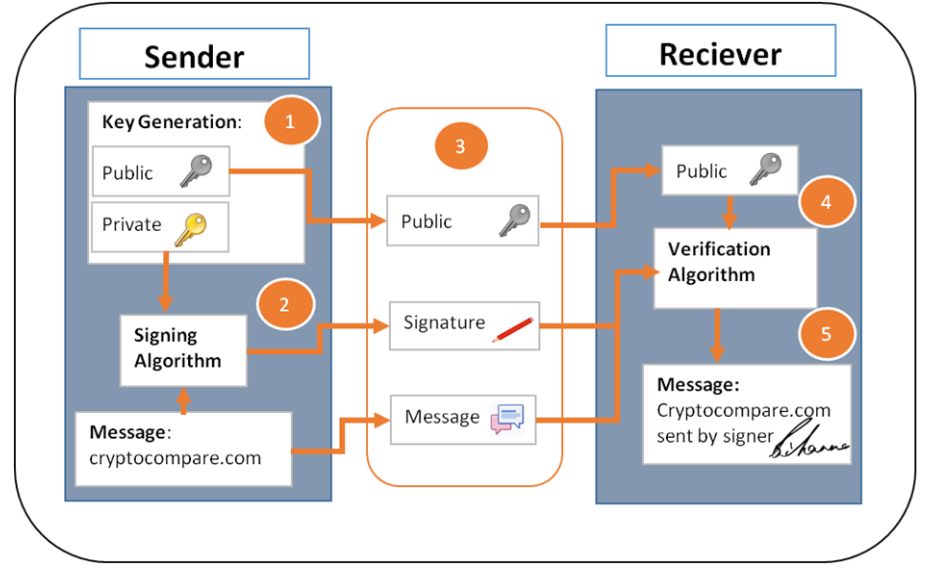
\includegraphics[scale = 0.35]{diagrams/transaction_diagram.png}
\end{center}

\newpage

The diagram above shows how an operation (here a transaction on the bitcoin protocol) is carried out.\\
1) You create a hash of the operation data (e.g. sender, receiver, message). Your private key is then used to sign this hash,
to create a digital signature.\\
2) You broadcast the operation data to the mining network, together with your digital signature and your public key.\\
3) Now, mining nodes can compute inexpensively whether your public key and your digital signature where made using the same private key.\\
4) If the transaction is valid, it is added to the aforementioned pool of operations to be placed in a block.

Let us now briefly discuss a few important applications of blockchain.
Earlier, I repeatedly mentioned \emph{operations} rather than \emph{transactions} intentionally.
When speaking about the infamous Bitcoin, it is accurate enough to speak of \emph{transactions} as its blockchain
only allows a small set of transaction-related operations.
Bitcoin and its blockchain thus form a cryptocurrency, with limited use beyond transacting at poor lentency.
RxCoin is concerned with later applications of blockchain technologies,
that aim to use their distributed databases for all sorts of operations beyong transactions.

In comes Ethereum...
Whereas Bitcoin restricts it blockchain to transaction-related operations, Ethereum has embraced all operations.
More precisely, they have implemented a turing-complete blockchain.
A system is said to be turing complete if it can be used to solve any computable problem.
Ethereum's blockchain is thus a platform rather than a cryptocurrency.
They designed a coding language that Ethereum mining software can interpret. 
A user is free broadcast any data and/or code to the platform, and as miners validate a block,
they execute this code to update the state of the database.
Codes, often referred to as \emph{smart contracts}, can call on other contracts, or be called upon.
Using this framework, anyone can create a application that uses Ethereum's decentralized database.
Today, most of the cryptocurrencies or ICOs you read about, have not implemented a blockchain themselves,
but rather, use Ethereum's blockchain.

RxCoin aims to disrupt the healthcare industry by introducing a blockchain devoted to healthcare-related operations.
One that would see its decentralized database bring transparency about this often too opaque industry,
and remove existing friction between manufacturers, prescribers and patients. 

